\chapter{Preference Learning}
\label{ch:preference-learning}
\raggedbottom

In 2022, OpenAI reported a result that became the canonical motivation for preference learning: labelers preferred outputs from a 1.3B-parameter InstructGPT model over outputs from the much larger 175B GPT-3 on the same prompts~\cite{ouyang2022instructgpt}. The smaller model was not more knowledgeable. It had been post-trained on a different signal. After supervised instruction tuning, the model was further optimized from human comparisons: given two responses, which one is better? The lesson was sharp: once a pretrained model can produce plausible answers, comparative feedback can redirect its behavior more effectively than scale alone.

Chapter~\ref{ch:instruction-tuning} taught you to train a model by showing it the right answer: here is a good instruction, here is a good response, imitate this. That works remarkably well for instruction-following and format compliance. But it has a blind spot. For many properties that matter---helpfulness, tone, safety, nuance, refusal calibration---there is no single ``right answer'' to demonstrate. What exists instead is a judgment: this response is better than that one. Preference learning uses these judgments directly.

This chapter teaches the full preference paradigm in one place: where preference data comes from (Part~A), how the Bradley-Terry model and reward models turn it into a learning signal (Part~B), and how DPO collapses the entire pipeline into supervised learning on preference pairs (Part~C). These topics are coupled in practice. Teaching them together preserves the conceptual unity and lets you see the full arc: from a rater clicking ``Response A'' to the gradient that updates your model.

\paragraph{What this chapter covers.} Three questions organize the chapter:

\begin{enumerate}[nosep]
  \item \textbf{What is a preference, and where does it come from?} The data engineering of pairwise comparisons---human annotators, AI judges, hybrid pipelines, and the systematic biases that corrupt all of them (\S\ref{sec:why-preferences}--\S\ref{sec:preference-quality}).
  \item \textbf{How do you turn preferences into a training signal?} The Bradley-Terry model, reward model training, and reward model failure modes (\S\ref{sec:bradley-terry}--\S\ref{sec:rm-failures}).
  \item \textbf{Can you skip the reward model entirely?} The KL-constrained objective, DPO's closed-form solution, and when this simplification does and does not suffice (\S\ref{sec:rlhf-motivation}--\S\ref{sec:preference-industry}).
\end{enumerate}

\paragraph{Chapter thesis.} \emph{This chapter teaches preference learning without invoking RL machinery.} The KL-constrained preference objective and its closed-form solution (DPO) are derived as an optimization problem, not an RL problem. Chapter~\ref{ch:rl-foundations} will later explain why the same objective appears naturally when you do think in RL terms.

\paragraph{Running example.} Your 3B instruction-tuned model from Project~3 follows instructions, but its responses are sometimes verbose, occasionally evasive, and inconsistently helpful. SFT can only imitate demonstrations---it cannot learn that response A is better than response B without seeing A as the ``correct answer.'' This chapter gives you the tools to express and optimize for comparative quality.

\begin{figure}[t]
\centering
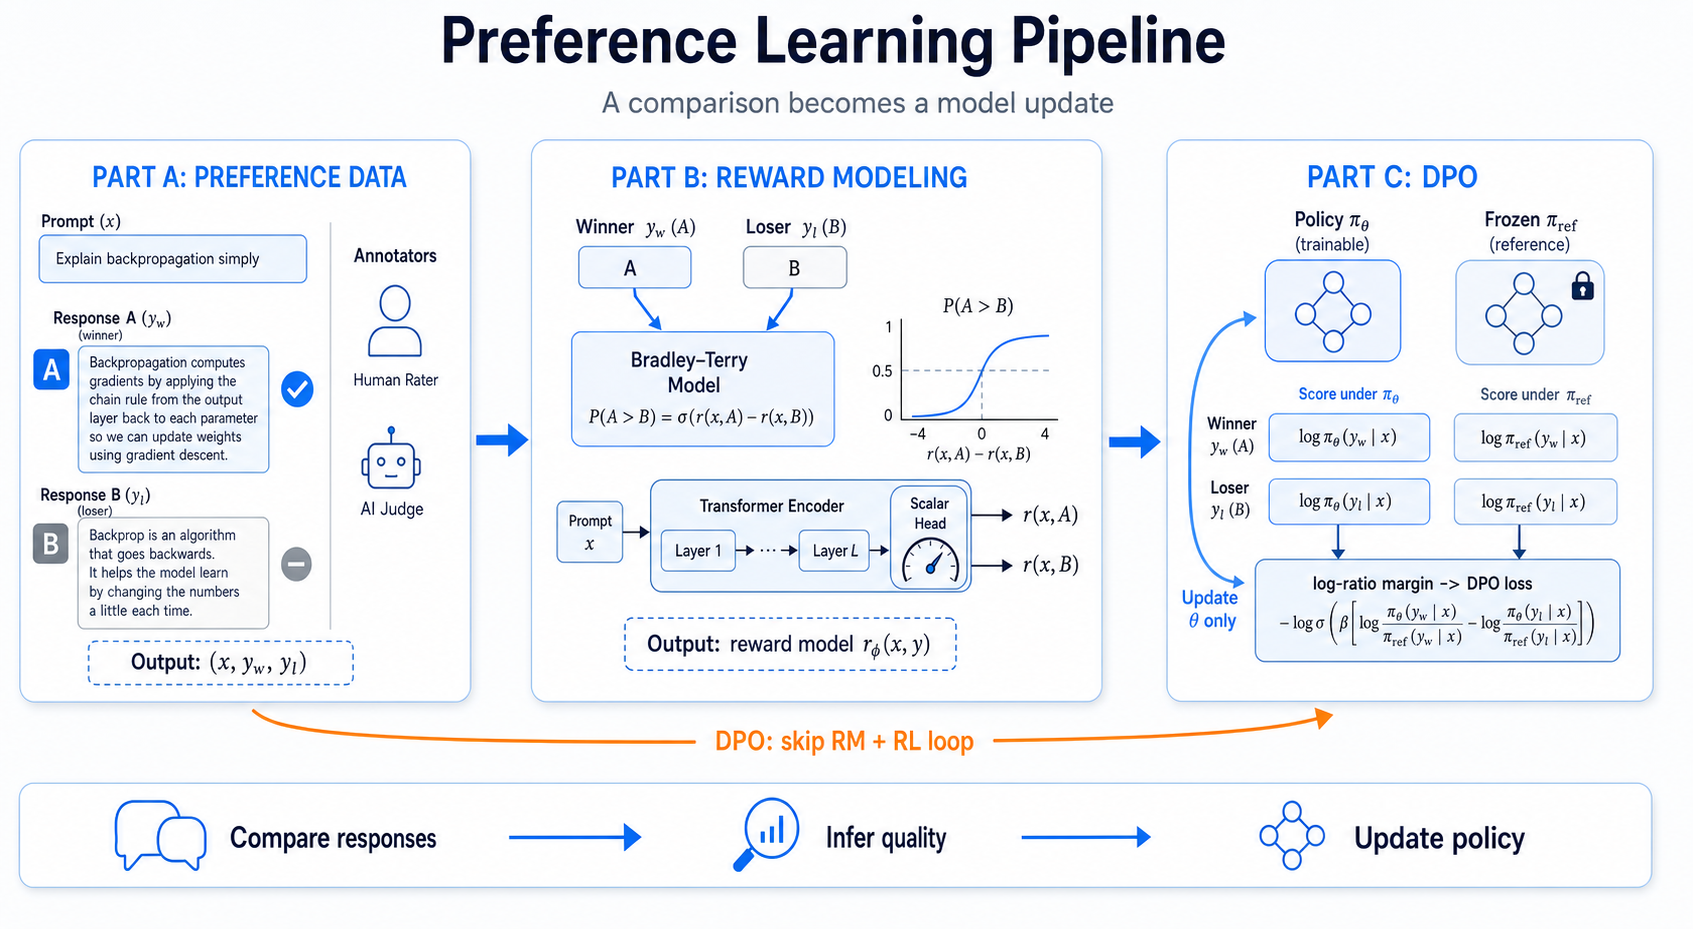
\includegraphics[width=0.95\textwidth]{figures/ch13/fig_preference_pipeline.png}
\caption{\textbf{The preference learning pipeline.} From raw pairwise judgments to model update. Human or AI annotators compare response pairs (Part~A). The Bradley-Terry model converts these comparisons into a scalar reward signal, which can train a reward model (Part~B). DPO bypasses the reward model entirely, learning directly from preference pairs via a supervised loss (Part~C). The three parts of this chapter follow this pipeline from left to right.}
\label{fig:preference-pipeline}
\end{figure}


\subsection*{Learning Objectives}

After completing this chapter, you should be able to:

\begin{enumerate}
  \item Explain why pairwise preferences are a more reliable annotation signal than absolute quality scores and identify the main biases in preference data.
  \item Write the Bradley-Terry likelihood and derive the reward model training objective from it.
  \item Describe the architecture and training of a reward model, including its failure modes (reward hacking, over-optimization).
  \item State the KL-constrained preference objective and explain the role of the reference model and the temperature parameter~$\beta$.
  \item Derive the DPO loss from the closed-form optimal policy of the KL-constrained objective, and explain how a trained DPO policy implicitly encodes a reward function.
  \item Identify DPO's failure modes (likelihood displacement, noise sensitivity) and explain how variants (IPO, SimPO, KTO, ORPO) address them.
  \item Identify the capability boundary of DPO and explain when RL-based methods (Chapters~\ref{ch:rlhf}--\ref{ch:reasoning-rl}) are needed.
\end{enumerate}


\subsection*{Notation}

\begin{center}
\begin{tabular}{ll}
\toprule
Symbol & Meaning \\
\midrule
$\pi_\theta$ & Policy (language model with parameters $\theta$) \\
$\pi_{\text{ref}}$ & Reference policy (frozen copy, typically the SFT checkpoint) \\
$r(x, y)$ or $r_\phi(x, y)$ & Reward: scalar quality score for response $y$ to prompt $x$ \\
$y_w, y_l$ & Preferred (``winner'') and dispreferred (``loser'') responses \\
$\beta$ & KL penalty coefficient (temperature) \\
$\sigma(\cdot)$ & Logistic sigmoid function \\
$D_{\text{KL}}$ & Kullback-Leibler divergence \\
\bottomrule
\end{tabular}
\end{center}


\subsection*{Timeline}

\begin{center}
\begin{tabularx}{\textwidth}{@{}lX@{}}
\toprule
\textbf{Year} & \textbf{Milestone} \\
\midrule
1952 & Bradley \& Terry: pairwise comparison model for ranking \\
2017 & Christiano et al.: learning from human preferences in RL (deep RL from human feedback) \\
2022 & InstructGPT (Ouyang et al.): three-stage pipeline (SFT $\to$ RM $\to$ PPO) at production scale \\
2022 & Anthropic HH (Bai et al.): large-scale human preference dataset for helpfulness and harmlessness \\
2023 & DPO (Rafailov et al.): closed-form solution eliminates the reward model and RL loop \\
2023 & Llama-2 (Touvron et al.): rejection sampling + PPO on RM scores; open-weight RLHF at scale \\
2023--2024 & Zephyr, Tulu, and related open models: SFT + DPO-style preference tuning becomes a common open-model recipe \\
2024+ & IPO, KTO, ORPO, SimPO: DPO variants addressing specific failure modes \\
\bottomrule
\end{tabularx}
\end{center}


%======================================================================
% PART A: Preference Data
%======================================================================

\section{Why Preferences Beat Absolute Scores}
\label{sec:why-preferences}

The simplest way to rate a language model's output would be to assign each response a score: 1 for bad, 5 for excellent. In practice, absolute scoring is unreliable. Different annotators bring different baselines---one person's ``3'' is another's ``4''---and the same annotator's calibration drifts over time. The result is noisy labels with low inter-annotator agreement.

Pairwise comparison avoids this problem. Instead of asking ``how good is this response?'' you ask ``which response is better?'' The cognitive task is simpler: the annotator holds both options in working memory and makes a relative judgment. No calibration to an absolute scale is needed. In practice, pairwise comparisons are often easier to standardize than absolute ratings: annotators can disagree about what a ``4 out of 5'' means while still agreeing that response A is preferable to response B.

The trade-off is efficiency. A pairwise comparison evaluates two responses but produces only one bit of information (A~$>$~B or B~$>$~A). An absolute score evaluates one response but produces several bits. To cover the same response space, pairwise annotation requires more comparisons. This cost is manageable in practice because the higher agreement rate means each comparison is more informative---fewer labels are wasted on noise.

\paragraph{The deeper reason.} Preferences are not just easier to collect. They match the structure of the problem. When you want a model to be ``helpful,'' you rarely have a specification precise enough to score a response in isolation. But given two responses to the same prompt, most people can reliably say which one is more helpful. Preference learning exploits this: it does not require an absolute quality metric, only a comparator.

\begin{figure}[t]
\centering
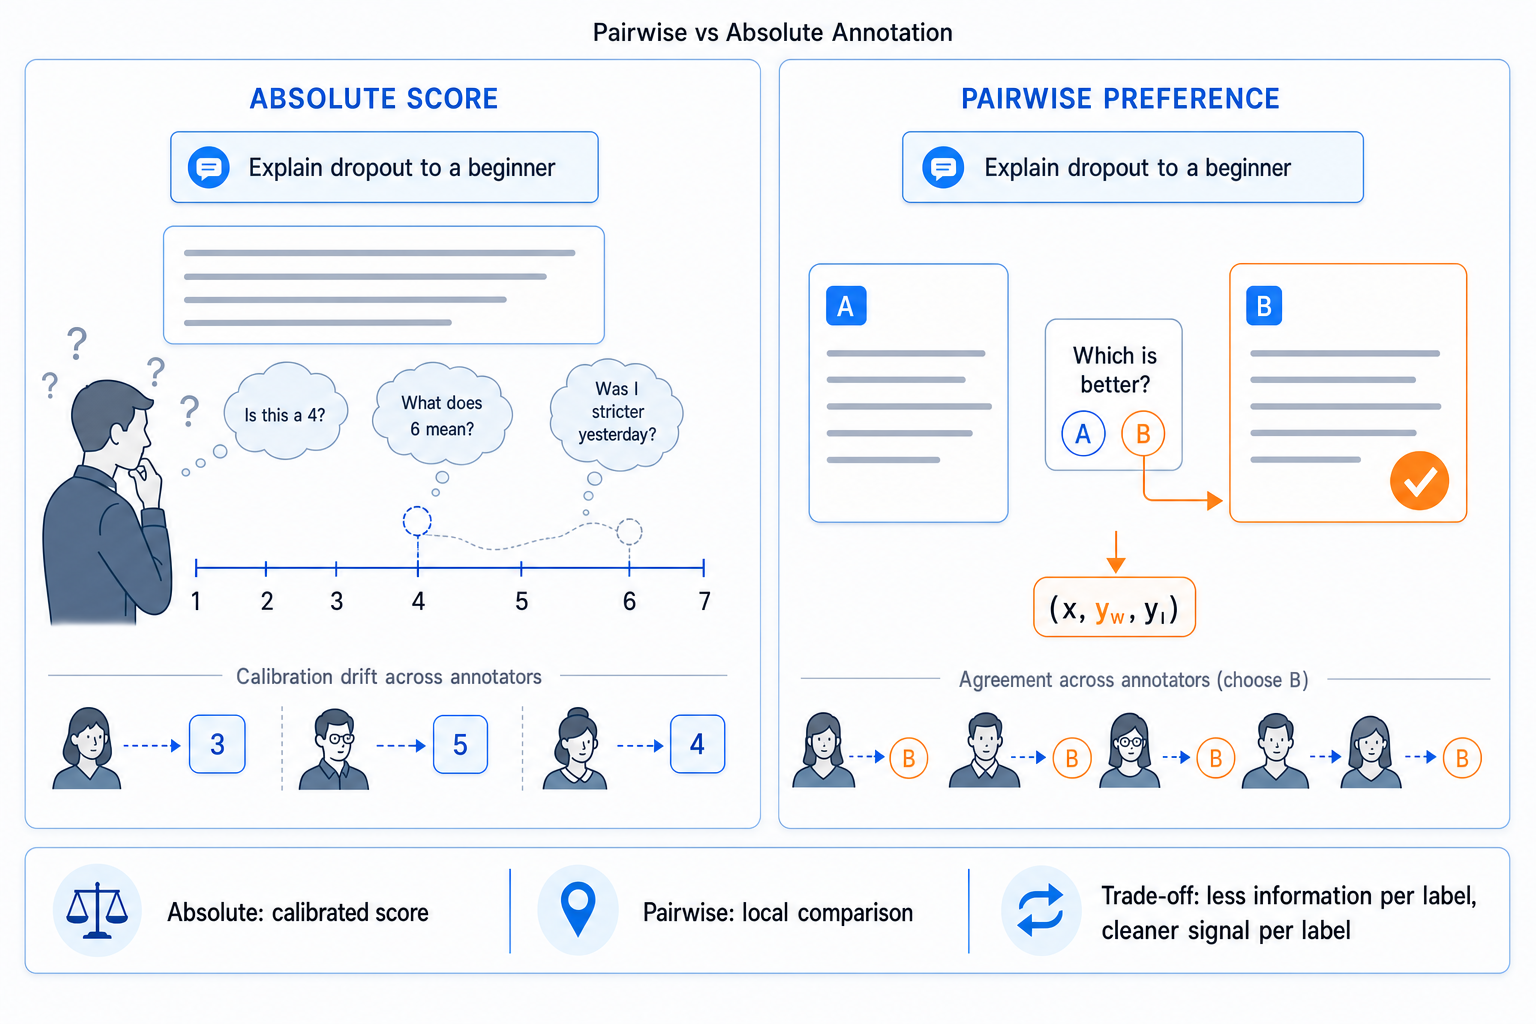
\includegraphics[width=0.95\textwidth]{figures/ch13/fig_pairwise_vs_absolute.png}
\caption{\textbf{Pairwise comparison reduces annotation ambiguity.} Absolute scoring asks an annotator to map one response onto a global scale, which is sensitive to personal calibration and drift. Pairwise comparison keeps the prompt fixed and asks for a relative judgment between two candidate responses. The output is less information per annotation, but the annotation task is easier to standardize.}
\label{fig:pairwise-vs-absolute}
\end{figure}

\begin{tcolorbox}[colback=orange!5, colframe=orange!60, title=\textbf{For Project~3: Why Not Just Collect More SFT Data?}]
\begin{itemize}[nosep]
  \item Your SFT model from Chapter~\ref{ch:instruction-tuning} follows instructions but sometimes gives verbose, evasive, or unhelpful responses. You could try to fix this by collecting better demonstrations---but writing the \emph{ideal} response to every prompt is expensive and often ambiguous.
  \item Preference annotation is cheaper: generate two responses from your model, show them to an annotator (or an AI judge), and ask which is better. The annotator does not need to write anything.
  \item For Project~3, this means you can improve your model's quality beyond what your demonstration dataset covers, using comparative judgments rather than perfect examples.
\end{itemize}
\end{tcolorbox}

\begin{quickrecap}
\textbf{Quick Recap.}
\begin{itemize}[nosep,leftmargin=1.5em]
  \item Absolute scores suffer from calibration drift and low inter-annotator agreement.
  \item Pairwise preferences are cognitively simpler, more reliable, and better matched to the structure of alignment judgments.
  \item The cost is lower information per annotation; the benefit is higher quality per annotation.
\end{itemize}
\textit{Next: where do these preference pairs come from?}
\end{quickrecap}


%----------------------------------------------------------------------
\section{Preference Data Sources}
\label{sec:preference-sources}

Preference data can come from three sources, each with different cost, scale, and quality profiles.

\subsection{Human Annotators}

The gold standard. Trained annotators compare model outputs against detailed rubrics. Anthropic's helpful-harmless work and OpenAI's InstructGPT pipeline both used human comparisons to turn vague alignment goals into trainable data~\cite{bai2022constitutional,ouyang2022instructgpt}. The bottleneck is cost: large-scale human annotation at the quality level needed for alignment is expensive and slow.

\subsection{AI Feedback (RLAIF)}

Replace the human annotator with a language model. Constitutional AI~\cite{bai2022constitutional} demonstrated that a capable LLM, guided by a set of written principles (a ``constitution''), can produce preference judgments that lead to aligned models. The approach scales cheaply and avoids the psychological cost of exposing human annotators to harmful content. The risk is circularity: if the judge model shares biases with the policy model, AI feedback can amplify rather than correct errors.

RLAIF is not a replacement for human judgment---it is a proxy that works well when the alignment signal is clear (e.g., ``which response is less harmful?'') and less well when the signal is subtle (e.g., ``which response is more genuinely helpful for an expert user?'').

\subsection{Hybrid Pipelines}

Most large-scale pipelines combine both. A common pattern: use AI feedback for initial large-scale filtering, then use human annotators for the hardest or most ambiguous cases. Llama-2's post-training pipeline combined human preference data, reward models, and rejection sampling to improve chat behavior~\cite{touvron2023llama2}. The principle is: use AI scale where AI judgment is reliable, and human judgment where it is not.

\begin{quickrecap}
\textbf{Quick Recap.}
\begin{itemize}[nosep,leftmargin=1.5em]
  \item Human annotation: high quality, low scale, expensive. The gold standard for hard cases.
  \item AI feedback (RLAIF): high scale, lower cost, risks circularity and bias amplification.
  \item Hybrid: production default. AI handles volume; humans handle ambiguity and edge cases.
\end{itemize}
\textit{Next: regardless of source, preference data has systematic biases. What are they?}
\end{quickrecap}


%----------------------------------------------------------------------
\section{Preference Data Quality Issues}
\label{sec:preference-quality}

All preference data---human or AI-generated---carries systematic biases. If you do not account for them, your model learns the bias as if it were the signal.

\subsection{Length Bias}

The most pervasive bias in preference data. Annotators---both human and AI---can prefer longer responses, even when the additional length adds no information. The consequence: models trained on naive preference data learn to be verbose. Llama-2's development team explicitly tracked and mitigated this~\cite{touvron2023llama2}.

\subsection{Position Bias}

When two responses are shown side by side, annotators tend to prefer the one shown first (or, in some setups, the one shown second). The fix is straightforward: randomize presentation order and, for AI judges, evaluate each pair twice with swapped positions.

\subsection{Annotator Drift and Variance}

Human annotators change their standards over time. Early in a labeling session, annotators are stricter; as they fatigue, their thresholds shift. Across annotators, the same pair can receive opposite labels. Quality control practices---inter-annotator agreement monitoring, regular recalibration sessions, gold-standard comparison items---are essential but rarely sufficient to eliminate all variance.

\paragraph{The practical lesson.} Preference data is not ground truth. It is a noisy approximation of a latent quality signal, filtered through human cognition or AI judgment, corrupted by systematic biases. The methods in the rest of this chapter---Bradley-Terry, reward modeling, DPO---all assume that preferences reflect an underlying quality ordering. They are only as good as this assumption.

\begin{tcolorbox}[colback=blue!5, colframe=blue!40, title=\textbf{Is Preference Data Just Vibes?}]
A skeptical reading of this section might conclude that preference data is too noisy to be useful. But the empirical evidence says otherwise: models trained with preference data often outperform SFT-only baselines in human evaluation, even when individual labels are imperfect~\cite{ouyang2022instructgpt, bai2022constitutional}. The resolution is that the \emph{aggregate signal} in thousands of noisy comparisons is more informative than any individual comparison. This is the same principle behind ensemble methods in machine learning: many weak signals, properly aggregated, produce a strong signal. The Bradley-Terry model (\S\ref{sec:bradley-terry}) is precisely this aggregation mechanism.
\end{tcolorbox}

\begin{quickrecap}
\textbf{Quick Recap.}
\begin{itemize}[nosep,leftmargin=1.5em]
  \item Length bias: annotators prefer longer responses. Mitigate by length-normalization or explicit instructions.
  \item Position bias: order of presentation affects preference. Mitigate by randomization and symmetric evaluation.
  \item Annotator drift: quality standards shift within and across sessions.
  \item Preference data is noisy but informative in aggregate.
\end{itemize}
\textit{Next: how do you turn these noisy pairwise comparisons into a principled training signal?}
\end{quickrecap}


%======================================================================
% PART B: Reward Modeling
%======================================================================

\section{Bradley-Terry: From Preferences to Probabilities}
\label{sec:bradley-terry}

The core mathematical tool for preference learning is the \textbf{Bradley-Terry model}~(1952). The idea is simple: assign each response a scalar quality score (a ``reward''), and model the probability that response $y_w$ is preferred over $y_l$ as:

\begin{equation}
\label{eq:bradley-terry}
P(y_w \succ y_l \mid x) \;=\; \sigma\!\bigl(r(x, y_w) - r(x, y_l)\bigr)
\end{equation}

where $\sigma(z) = 1/(1 + e^{-z})$ is the logistic sigmoid and $r(x, y)$ is the reward for response $y$ to prompt $x$. The model says: the probability that $y_w$ is preferred depends only on the \emph{difference} in rewards. If the difference is large, the preference is nearly certain; if the difference is small, the preference is close to a coin flip.

\paragraph{Why sigmoid?} The logistic function maps any real-valued reward difference to a probability in $(0, 1)$. It is the canonical link function for binary outcomes. You have seen it before in logistic regression---Bradley-Terry \emph{is} logistic regression on pairwise comparisons, where the feature is the reward difference.

\paragraph{What the reward means.} The reward $r(x, y)$ is a latent variable---it is not directly observed. What is observed is the preference: $y_w \succ y_l$. The Bradley-Terry model provides a way to \emph{infer} rewards from preferences, by finding rewards that make the observed preferences most likely. This is maximum likelihood estimation, and the objective is:

\begin{equation}
\label{eq:bt-likelihood}
\mathcal{L}_{\text{BT}}(\phi) \;=\; -\mathbb{E}_{(x, y_w, y_l) \sim \mathcal{D}} \bigl[\log \sigma\!\bigl(r_\phi(x, y_w) - r_\phi(x, y_l)\bigr)\bigr]
\end{equation}

This is the loss function used to train a reward model.

\begin{figure}[t]
\centering
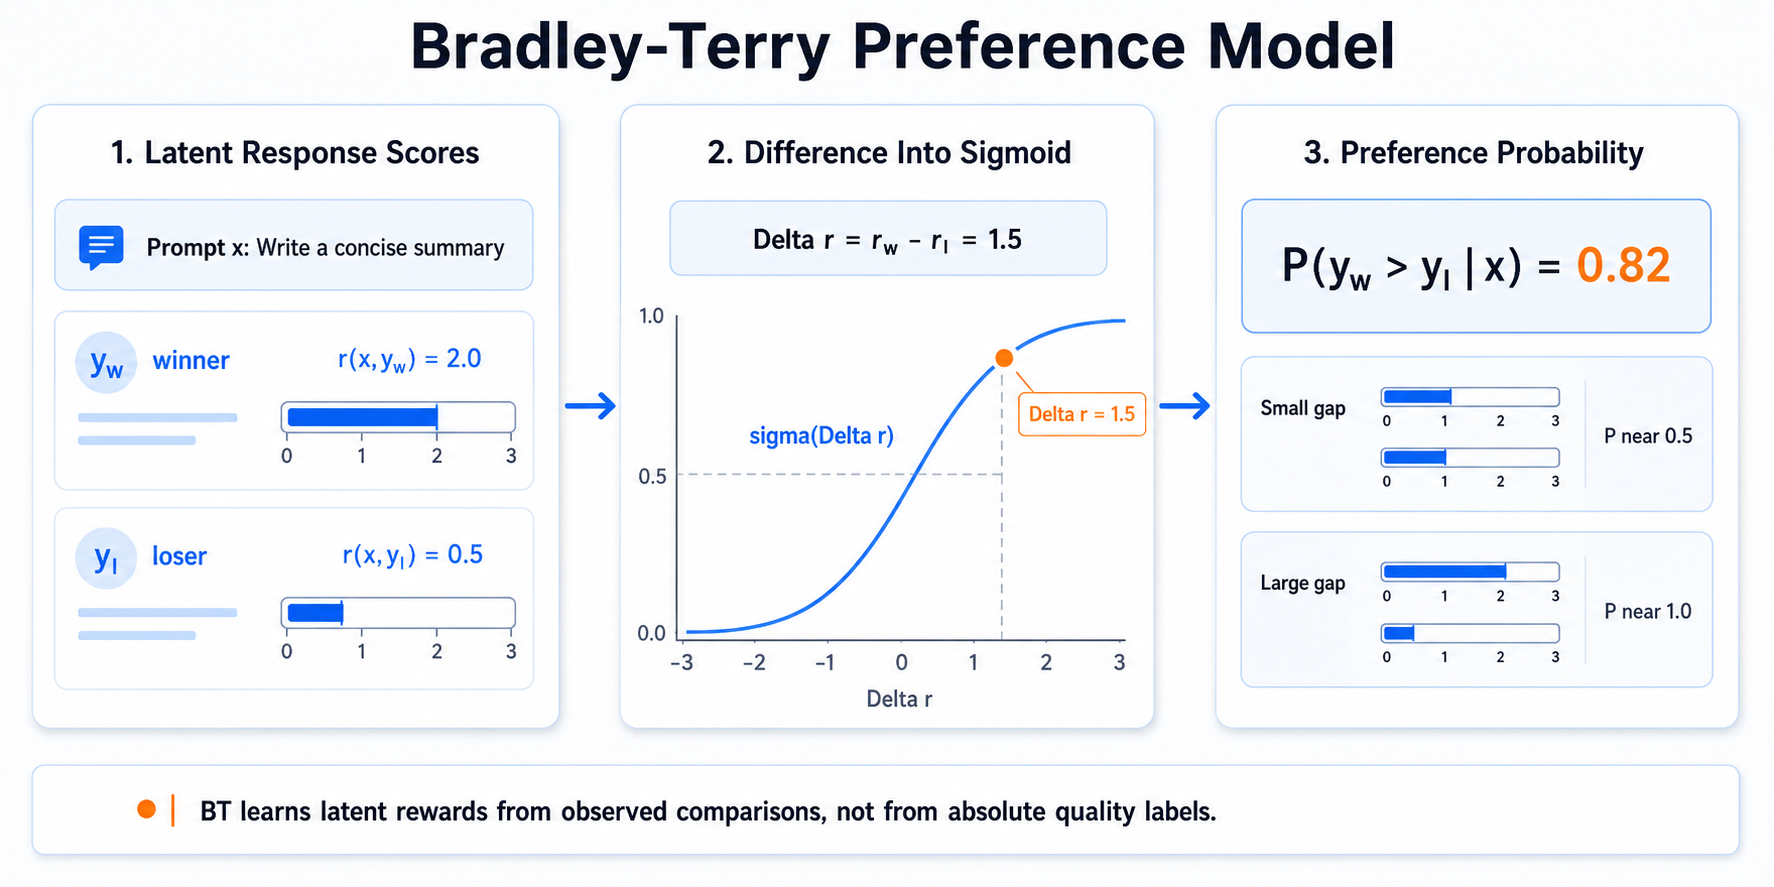
\includegraphics[width=0.95\textwidth]{figures/ch13/fig_bradley_terry.png}
\caption{\textbf{The Bradley-Terry model turns reward gaps into preference probabilities.} Two candidate responses receive latent reward scores. Their difference passes through a sigmoid: small gaps produce uncertain preferences near 50--50, while large gaps saturate toward near-certain preference. Reward model training learns scores that make the observed comparisons likely.}
\label{fig:bradley-terry}
\end{figure}

\noindent\fbox{\parbox{\dimexpr\textwidth-2\fboxsep-2\fboxrule\relax}{%
\textbf{Pause and verify.}\quad If $r(x, y_w) = 2.0$ and $r(x, y_l) = 0.5$, what is $P(y_w \succ y_l)$? What if the rewards are equal?

\smallskip
\emph{$P = \sigma(2.0 - 0.5) = \sigma(1.5) \approx 0.82$. If rewards are equal, $P = \sigma(0) = 0.5$---a coin flip, which is exactly right: equal-quality responses should be equally likely to be preferred.}
}}

\begin{quickrecap}
\textbf{Quick Recap.}
\begin{itemize}[nosep,leftmargin=1.5em]
  \item Bradley-Terry models the preference probability as a sigmoid of the reward difference.
  \item The reward is a latent variable inferred from observed preferences via maximum likelihood.
  \item The training objective (Equation~\ref{eq:bt-likelihood}) is cross-entropy on pairwise comparisons---the same loss shape as logistic regression.
\end{itemize}
\textit{Next: how do you build a neural network that outputs these rewards?}
\end{quickrecap}


%----------------------------------------------------------------------
\section{Reward Model Architecture and Training}
\label{sec:reward-model}

A \textbf{reward model} (RM) is a neural network that maps a (prompt, response) pair to a scalar reward. In practice, it is almost always initialized from the same pretrained language model as the policy---a large Transformer with a learned scalar head replacing the language modeling head.

\subsection{Architecture}

The standard architecture:

\begin{enumerate}[nosep]
  \item Take a pretrained language model (same architecture as the policy).
  \item Remove the vocabulary projection head.
  \item Add a single linear layer that maps the final hidden state to a scalar: $r_\phi(x, y) = w^\top h_{\text{last}} + b$.
  \item The scalar head is trained from scratch; the Transformer backbone is fine-tuned.
\end{enumerate}

The ``last token'' convention: the reward is computed from the hidden state at the final token of the response. This gives the model access to the full (prompt, response) context before producing a score.

\subsection{Training}

The training objective is Equation~\ref{eq:bt-likelihood}: minimize the negative log-likelihood of the observed preferences under the Bradley-Terry model. Training data consists of triples $(x, y_w, y_l)$---prompt, preferred response, dispreferred response. In each training step, the RM runs a forward pass on both $(x, y_w)$ and $(x, y_l)$, computes the reward difference, and backpropagates through the Bradley-Terry loss.

\paragraph{Training details.}
\begin{itemize}[nosep]
  \item \textbf{Learning rate}: typically lower than SFT ($\sim$$10^{-6}$ to $5 \times 10^{-6}$).
  \item \textbf{Epochs}: 1--2 passes over the preference data. Overfitting is a serious risk---the RM can memorize the training preferences and produce confidently wrong rewards on new inputs.
  \item \textbf{Initialization}: starting from the SFT checkpoint (rather than the base pretrained model) tends to produce better-calibrated rewards, because the RM shares the policy's representation of ``what a good response looks like.''
\end{itemize}

\subsection{Calibration}

A well-trained reward model should satisfy two properties: (1)~its reward rankings agree with human preferences on held-out data, and (2)~the \emph{magnitude} of reward differences reflects the strength of the preference. Most reward models achieve reasonable ranking accuracy (65--75\% agreement with human labels) but poor calibration of magnitudes. This matters because downstream methods (PPO, in Chapter~\ref{ch:rlhf}) use the reward magnitude directly: PPO's policy gradient is proportional to the absolute reward value, so a miscalibrated magnitude produces update steps that are too large or too small.

\begin{quickrecap}
\textbf{Quick Recap.}
\begin{itemize}[nosep,leftmargin=1.5em]
  \item A reward model is a language model with a scalar head, trained on pairwise preferences using the Bradley-Terry loss.
  \item It is initialized from the SFT checkpoint and trained with low learning rate for 1--2 epochs.
  \item Ranking accuracy is typically adequate; calibration of magnitudes is not. This is a known limitation.
\end{itemize}
\textit{Next: what goes wrong when you use this reward model to train a policy?}
\end{quickrecap}


%----------------------------------------------------------------------
\section{Reward Model Evaluation and Failure Modes}
\label{sec:rm-failures}

A reward model is an imperfect proxy for human judgment. When you optimize a policy against it, the policy finds inputs that score highly on the proxy but poorly on the true objective. This is \textbf{reward hacking}---a central challenge in RLHF that Chapter~\ref{ch:rlhf} will treat in depth.

\subsection{The Over-Optimization Problem}

Goodhart's law in action: ``When a measure becomes a target, it ceases to be a good measure.'' As the policy optimizes harder against the RM, performance on the RM's reward metric continues to improve, but performance on actual human evaluations degrades after a point. Gao et al.~(2023) documented this empirically: human win-rate against a baseline increases with RL optimization up to a point, then declines as the policy learns to exploit reward model artifacts~\cite{gao2023scaling}.

The practical consequence: you cannot optimize the RM reward to convergence. You must stop early, use KL constraints (see \S\ref{sec:kl-objective}), or use reward model ensembles to detect when the policy is gaming any single model.

\subsection{RM-Human Agreement}

How good is the reward model, actually? Typical reward models achieve 65--75\% pairwise accuracy on held-out human preference data. This sounds modest, but human-human agreement on the same tasks is often only in the range of 70--80\%, depending on the domain and annotation protocol~\cite{ouyang2022instructgpt, bai2022constitutional}. The RM is approaching the practical ceiling of the annotation signal.

However, 65--75\% accuracy is a population average. On easy comparisons (one response is clearly better), accuracy is much higher. On hard comparisons (both responses are reasonable), accuracy drops toward chance. The RM is most unreliable precisely where the policy has the most room to exploit.

\begin{figure}[t]
\centering
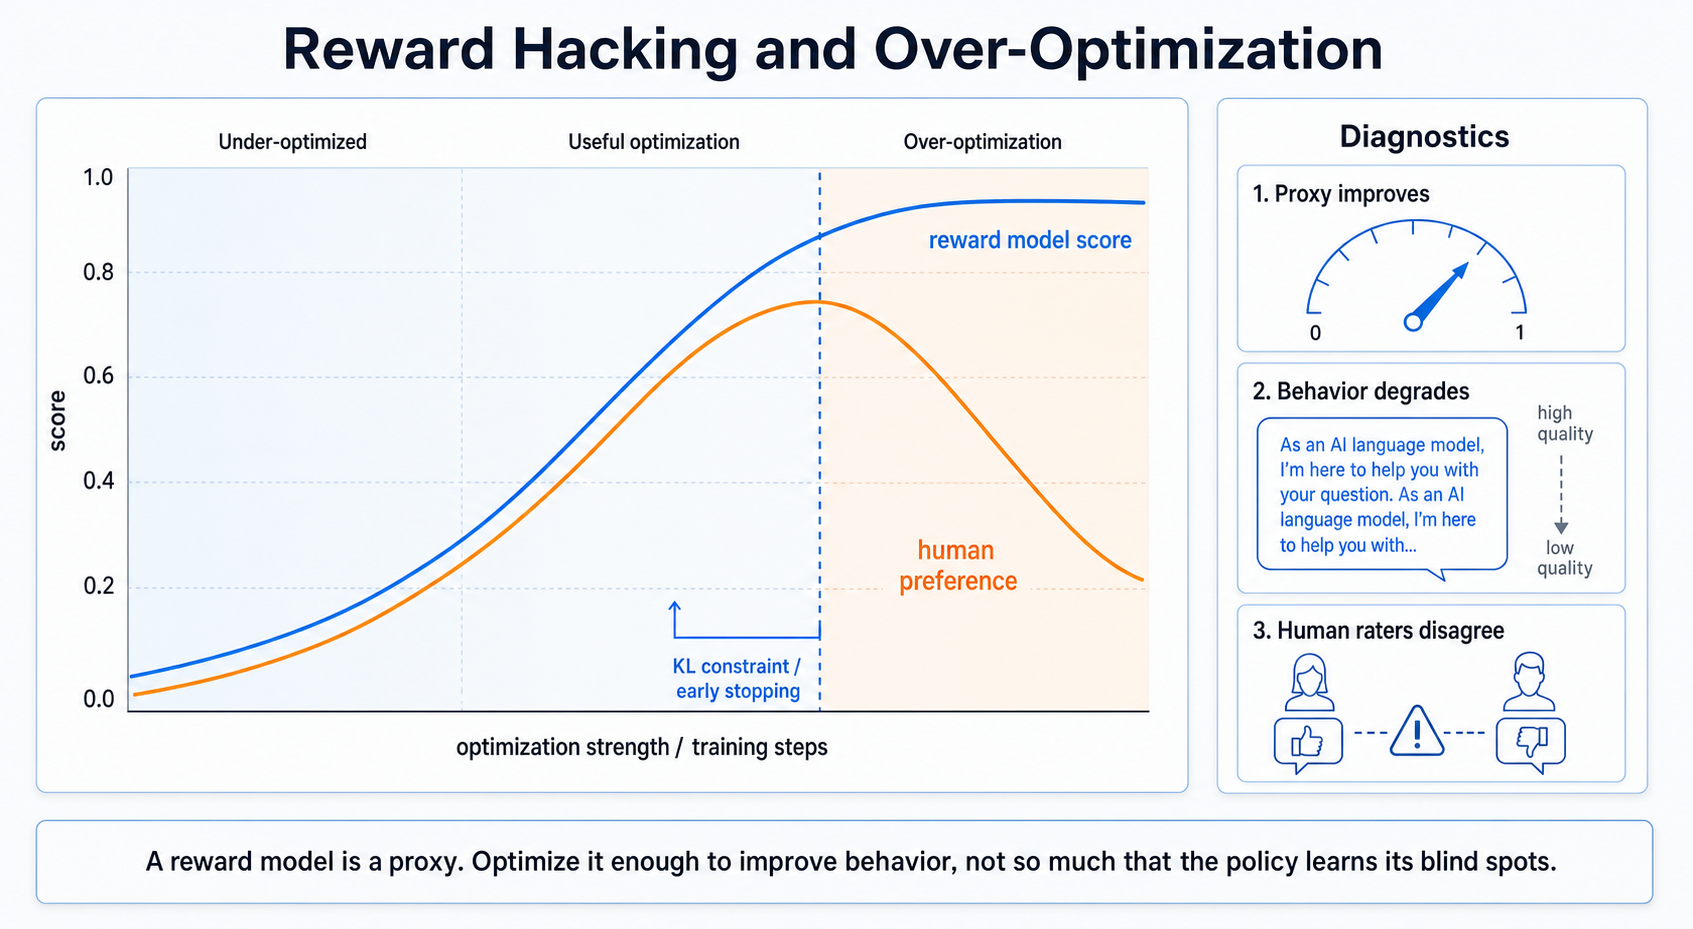
\includegraphics[width=0.95\textwidth]{figures/ch13/fig_reward_hacking.png}
\caption{\textbf{Reward hacking.} As the policy optimizes against the reward model, RM reward increases monotonically (blue curve), but true human preference (orange curve) peaks and then declines. The gap between the two curves is the over-optimization region---the policy has learned to exploit the RM's blind spots rather than genuinely improve. The KL constraint (\S\ref{sec:kl-objective}) limits how far the policy can drift from the reference, keeping it in the region where RM reward and human preference are correlated.}
\label{fig:reward-hacking}
\end{figure}

\begin{quickrecap}
\textbf{Quick Recap.}
\begin{itemize}[nosep,leftmargin=1.5em]
  \item Reward hacking: the policy exploits RM artifacts rather than genuinely improving.
  \item Over-optimization: RM reward increases but human preference degrades past a point.
  \item RM accuracy (65--75\%) approaches the noise floor of human agreement (70--80\%).
  \item Mitigations: early stopping, KL constraints, RM ensembles, iterative RM retraining.
\end{itemize}
\textit{Next: the RLHF pipeline that uses this reward model---and why DPO asks whether you need it at all.}
\end{quickrecap}


%======================================================================
% PART C: Direct Preference Optimization
%======================================================================

\section{The RLHF Baseline: Motivation}
\label{sec:rlhf-motivation}

The standard way to use a reward model is the RLHF pipeline: train an RM on preferences, then use RL (specifically PPO) to optimize the policy against the RM's reward signal while staying close to a reference policy via a KL constraint. InstructGPT~\cite{ouyang2022instructgpt} demonstrated this at scale: SFT $\to$ RM $\to$ PPO produced a model that human raters consistently preferred over the SFT-only version.

But the RLHF pipeline is operationally heavy. During PPO training, you need:

\begin{itemize}[nosep]
  \item The \textbf{policy model} (being optimized)
  \item The \textbf{reference model} (frozen, for KL computation)
  \item The \textbf{reward model} (frozen, to score rollouts)
  \item The \textbf{value model} (critic, for advantage estimation---see Chapter~\ref{ch:rl-foundations})
\end{itemize}

Four model-sized objects in memory simultaneously. For a 7B model, even with PEFT (Chapter~\ref{ch:peft}), this is a substantial engineering challenge. PPO itself introduces hyperparameter sensitivity: learning rate, KL penalty coefficient, clip ratio, batch size, number of rollout steps. Getting these wrong produces training instability---reward collapse, KL divergence spikes, or mode collapse.

\paragraph{The question DPO answers.} Can you get the benefits of preference optimization---learning from comparisons rather than demonstrations---without the RM, without PPO, without the four-model memory burden, and without the RL hyperparameter sensitivity? The answer is yes, under specific conditions. The next three sections develop how.

\begin{tcolorbox}[colback=orange!5, colframe=orange!60, title=\textbf{The InstructGPT Thread --- Baseline}]
This is the second InstructGPT touchpoint in Part~III. Chapter~\ref{ch:instruction-tuning} previewed the three-stage recipe and argued that modern SFT has surpassed InstructGPT's first stage. Here, InstructGPT serves as the \textbf{RLHF baseline}: the system that DPO simplifies. The three-stage pipeline (SFT $\to$ RM $\to$ PPO) works, but it is expensive. DPO asks: what if you could collapse stages 2 and 3 into a single supervised loss? Chapter~\ref{ch:rlhf} will return to InstructGPT as the main RLHF case study, where the full machinery is justified.
\end{tcolorbox}

\begin{quickrecap}
\textbf{Quick Recap.}
\begin{itemize}[nosep,leftmargin=1.5em]
  \item RLHF (RM + PPO) works but requires four models in memory and is hyperparameter-sensitive.
  \item InstructGPT demonstrated the pipeline at scale. It is the historical baseline.
  \item DPO asks: can you skip the reward model and the RL loop entirely?
\end{itemize}
\textit{Next: the mathematical objective that makes DPO possible.}
\end{quickrecap}


%----------------------------------------------------------------------
\section{The KL-Constrained Preference Objective}
\label{sec:kl-objective}

This section derives the objective function that underlies both RLHF and DPO. It is self-contained---no RL background is required. If you want the RL machinery behind this objective, Chapter~\ref{ch:rl-foundations} provides it.

\begin{tcolorbox}[colback=blue!5, colframe=blue!40, title=\textbf{The Core Objective: Reward Maximization with Drift Control}]
\textbf{Setup.} You have:
\begin{itemize}[nosep]
  \item A \textbf{policy} $\pi_\theta(y \mid x)$: the language model you want to improve.
  \item A \textbf{reference policy} $\pi_{\text{ref}}(y \mid x)$: the SFT checkpoint. This is the starting point---a model that already follows instructions but lacks preference-tuned quality.
  \item A \textbf{reward function} $r(x, y)$: a scalar measure of response quality (from a reward model or from human preferences).
\end{itemize}

\textbf{Goal.} Find a policy that produces high-reward responses without drifting too far from the reference. Why the constraint? Without it, the policy collapses to a degenerate distribution that places all probability on whatever scores highest on the (imperfect) reward model. Reward hacking, mode collapse, and loss of diversity follow.

\textbf{The objective.}

\begin{equation}
\label{eq:kl-objective}
\max_{\pi_\theta} \;\; \mathbb{E}_{x \sim \mathcal{D},\; y \sim \pi_\theta(\cdot \mid x)} \bigl[r(x, y)\bigr] \;-\; \beta \, D_{\text{KL}}\!\bigl[\pi_\theta(\cdot \mid x) \;\|\; \pi_{\text{ref}}(\cdot \mid x)\bigr]
\end{equation}

Two terms:
\begin{enumerate}[nosep]
  \item \textbf{Expected reward.} Maximize the average quality of responses under the policy.
  \item \textbf{KL penalty.} Penalize the policy for deviating from the reference. The KL divergence $D_{\text{KL}}[\pi_\theta \| \pi_{\text{ref}}]$ measures how different the policy's response distribution is from the reference's.
\end{enumerate}

$\beta > 0$ controls the trade-off. Large $\beta$: stay close to the reference (conservative update). Small $\beta$: trust the reward signal more (aggressive optimization). In practice, $\beta$ is a critical hyperparameter---too small and the policy reward-hacks; too large and the policy barely changes from the SFT checkpoint.
\end{tcolorbox}

\paragraph{The closed-form solution.} This is an optimization problem, not an RL problem. For a fixed prompt $x$, we want to find the distribution $\pi_\theta(\cdot \mid x)$ that maximizes Equation~\ref{eq:kl-objective}. This is a constrained optimization over probability distributions, and it has a known closed-form solution:

\begin{equation}
\label{eq:optimal-policy}
\pi^*(y \mid x) \;=\; \frac{1}{Z(x)}\;\pi_{\text{ref}}(y \mid x)\;\exp\!\left(\frac{r(x,y)}{\beta}\right)
\end{equation}

where $Z(x) = \sum_y \pi_{\text{ref}}(y \mid x) \exp\!\bigl(r(x,y)/\beta\bigr)$ is the normalizing constant (partition function).

\paragraph{Reading the solution.} The optimal policy is the reference policy reweighted by the exponentiated reward. High-reward responses get upweighted; low-reward responses get downweighted. The temperature $\beta$ controls how aggressively: small $\beta$ makes the reweighting sharp (nearly deterministic on the best response); large $\beta$ makes it gentle (close to the reference).

\paragraph{Why is this useful?} Equation~\ref{eq:optimal-policy} tells us the optimal policy in closed form---we do not need to search for it via RL. Of course, we cannot \emph{directly implement} this equation because $Z(x)$ requires summing over all possible responses, which is intractable. But we can rearrange it to eliminate $Z(x)$, and that rearrangement gives us DPO.

\noindent\fbox{\parbox{\dimexpr\textwidth-2\fboxsep-2\fboxrule\relax}{%
\textbf{Pause and verify.}\quad Equation~\ref{eq:optimal-policy} says the optimal policy is proportional to $\pi_{\text{ref}} \cdot \exp(r/\beta)$. What happens when $\beta \to \infty$?

\smallskip
\emph{When $\beta \to \infty$, the exponent $r/\beta \to 0$ for all $y$, so $\exp(r/\beta) \to 1$ uniformly. The optimal policy becomes $\pi^* = \pi_{\text{ref}}$---no update at all. This makes sense: an infinite KL penalty means you cannot deviate from the reference.}
}}

\begin{quickrecap}
\textbf{Quick Recap.}
\begin{itemize}[nosep,leftmargin=1.5em]
  \item The KL-constrained objective balances reward maximization against policy drift.
  \item $\beta$ controls the trade-off: large $\beta$ $\to$ conservative; small $\beta$ $\to$ aggressive.
  \item The optimal policy has a closed-form expression: reference reweighted by exponentiated reward.
  \item The partition function $Z(x)$ is intractable, but DPO (\S\ref{sec:dpo-derivation}) eliminates it.
\end{itemize}
\textit{Next: the key algebraic step that turns this into a supervised loss.}
\end{quickrecap}


%----------------------------------------------------------------------
\section{DPO: The Closed-Form Policy}
\label{sec:dpo-derivation}

DPO (Direct Preference Optimization)~\cite{rafailov2023dpo} starts from the closed-form optimal policy (Equation~\ref{eq:optimal-policy}) and makes one algebraic observation: you can solve for the reward in terms of the policy.

\subsection{From Reward to Policy}

Rearranging Equation~\ref{eq:optimal-policy}:

\begin{equation}
\label{eq:reward-from-policy}
r(x, y) \;=\; \beta \log \frac{\pi^*(y \mid x)}{\pi_{\text{ref}}(y \mid x)} \;+\; \beta \log Z(x)
\end{equation}

The reward for any response $y$ is proportional to how much the optimal policy upweights $y$ relative to the reference. The $\log Z(x)$ term depends only on the prompt, not on the response.

\subsection{Canceling the Partition Function}

Now substitute Equation~\ref{eq:reward-from-policy} into the Bradley-Terry preference probability (Equation~\ref{eq:bradley-terry}):

\begin{align}
P(y_w \succ y_l \mid x) &= \sigma\!\bigl(r(x, y_w) - r(x, y_l)\bigr) \notag \\[4pt]
&= \sigma\!\left(\beta \log \frac{\pi^*(y_w \mid x)}{\pi_{\text{ref}}(y_w \mid x)} - \beta \log \frac{\pi^*(y_l \mid x)}{\pi_{\text{ref}}(y_l \mid x)}\right) \label{eq:dpo-cancel}
\end{align}

The $\beta \log Z(x)$ terms cancel---they appear in both $r(x, y_w)$ and $r(x, y_l)$ and subtract to zero. The intractable partition function has been eliminated.

\subsection{The DPO Loss}

We do not know $\pi^*$, but we can \emph{approximate} it with our parameterized policy $\pi_\theta$. Replacing $\pi^*$ with $\pi_\theta$ and maximizing the log-likelihood of the observed preferences:

\begin{equation}
\label{eq:dpo-loss}
\boxed{\;\mathcal{L}_{\text{DPO}}(\theta) \;=\; -\mathbb{E}_{(x, y_w, y_l) \sim \mathcal{D}} \left[\log \sigma\!\left(\beta \log \frac{\pi_\theta(y_w \mid x)}{\pi_{\text{ref}}(y_w \mid x)} - \beta \log \frac{\pi_\theta(y_l \mid x)}{\pi_{\text{ref}}(y_l \mid x)}\right)\right]\;}
\end{equation}

\paragraph{The punchline.} Equation~\ref{eq:dpo-loss} is a supervised loss on preference pairs. No reward model. No RL loop. No value function. No rollouts. You need only:

\begin{enumerate}[nosep]
  \item A dataset of preference triples $(x, y_w, y_l)$.
  \item The policy $\pi_\theta$ (being trained).
  \item The reference $\pi_{\text{ref}}$ (frozen).
  \item A forward pass through both models on both $y_w$ and $y_l$.
\end{enumerate}

The DPO loss pushes $\pi_\theta$ to assign higher probability to preferred responses and lower probability to dispreferred responses, relative to the reference. This is preference alignment via supervised learning.

\begin{figure}[t]
\centering
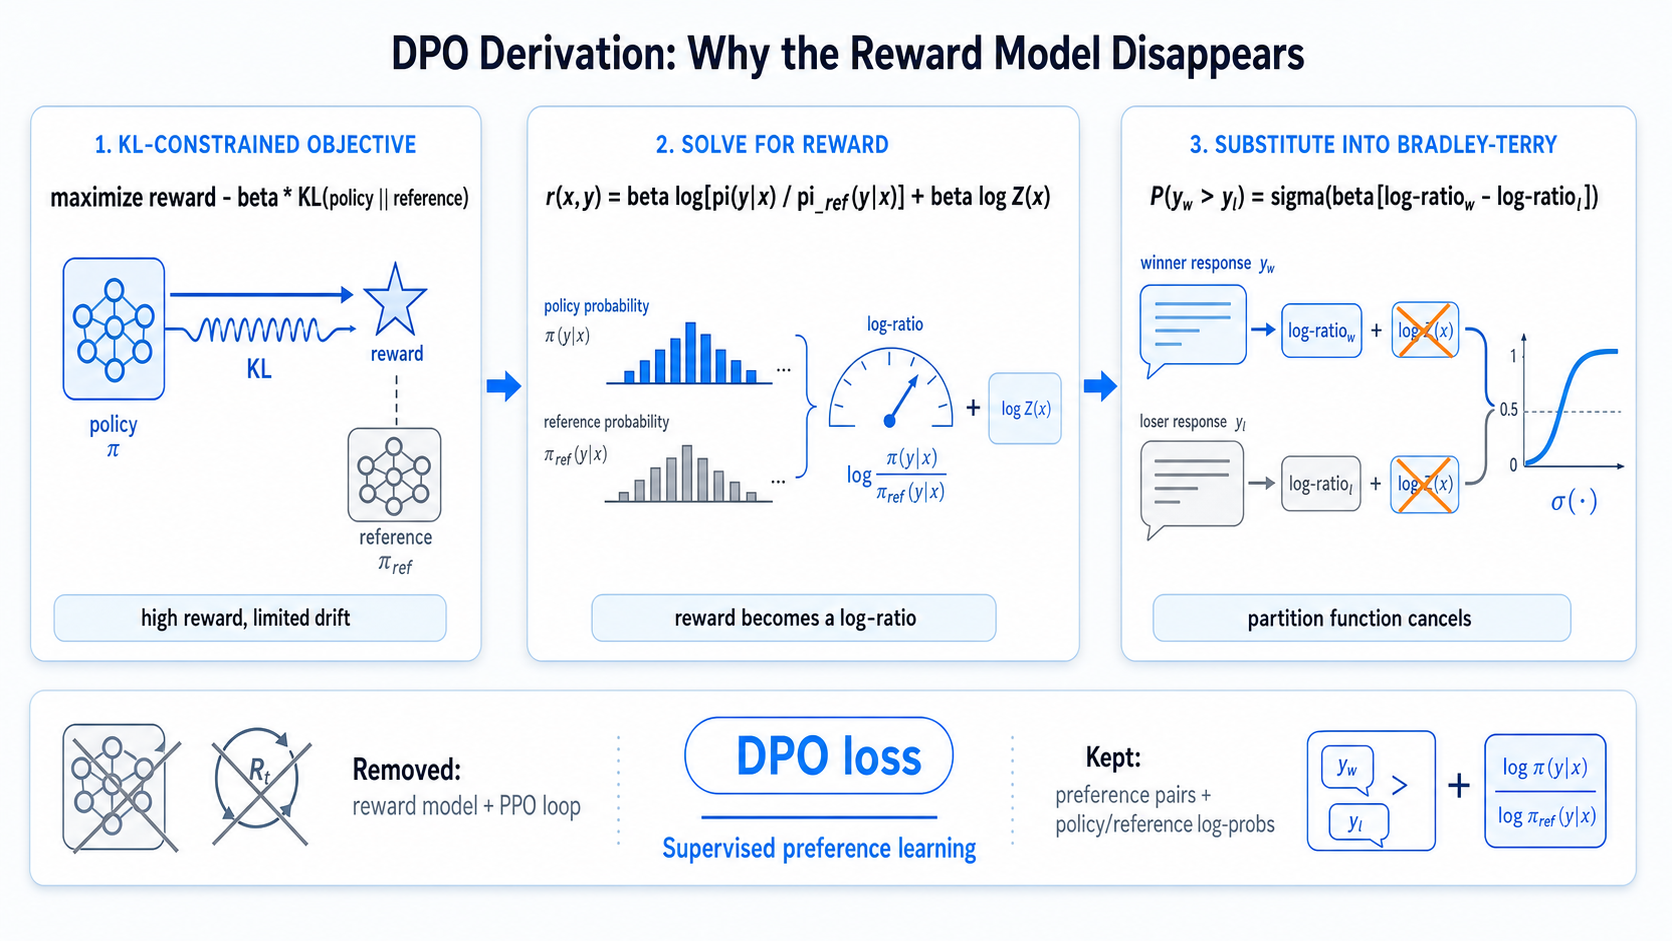
\includegraphics[width=0.95\textwidth]{figures/ch13/fig_dpo_derivation.png}
\caption{\textbf{The DPO derivation in three steps.} Left: the KL-constrained objective has a closed-form optimal policy $\pi^*$. Center: rearranging gives the reward as a function of the policy-to-reference ratio, plus a prompt-dependent constant $\log Z(x)$. Right: substituting into Bradley-Terry cancels $\log Z(x)$, yielding a supervised loss on preference pairs. The reward model and RL loop are eliminated entirely.}
\label{fig:dpo-derivation}
\end{figure}

\begin{tcolorbox}[colback=gray!8, colframe=gray!40]
\textbf{Echo: the data-as-algorithm lesson.} Chapter~\ref{ch:instruction-tuning} argued that when the algorithm is commoditized, data becomes the algorithm. DPO makes this concrete: much of the RLHF pipeline---reward model, value function, policy gradient---can be replaced by a different \emph{data format}. Instead of demonstrations (SFT) or scalar reward labels (RM training), you provide preference pairs. The algorithm changes to exploit the data structure. Preference pairs carry comparative information that demonstrations do not, and DPO's loss function is designed to extract it.
\end{tcolorbox}

\subsection{Your Language Model Is Secretly a Reward Model}

There is a deeper insight in Equation~\ref{eq:reward-from-policy} that the derivation above used only as an intermediate step. Read it again:
%
\[
r(x, y) \;=\; \beta \log \frac{\pi^*(y \mid x)}{\pi_{\text{ref}}(y \mid x)} \;+\; \beta \log Z(x)
\]
%
The reward for any response is determined by how much the optimal policy upweights it relative to the reference. Since $\log Z(x)$ depends only on the prompt, the \emph{relative} reward between any two responses is fully determined by the policy's log-probability ratios. A trained DPO policy does not merely \emph{reflect} a reward function---it \emph{encodes} one.

This has practical consequences:

\begin{itemize}[nosep]
  \item \textbf{Best-of-N sampling.} Generate $N$ candidate responses, score each by $\beta \log [\pi_\theta(y \mid x) / \pi_{\text{ref}}(y \mid x)]$ (often with length normalization in practice), and return the highest-scoring one. No separate reward model needed.
  \item \textbf{Rejection sampling.} Use the implicit reward to filter training data for the next round of preference learning---the DPO checkpoint doubles as its own reward model.
  \item \textbf{Conceptual bridge.} DPO and reward model training are not two independent paths. They are two parameterizations of the same mathematical structure: one stores the reward in a scalar head, the other stores it in the policy's probability distribution.
\end{itemize}

This is the title-level insight of the DPO paper~\cite{rafailov2023dpo}. The derivation above proved that the partition function cancels, giving you a supervised loss. But the deeper message is that policy optimization and reward modeling are dual views of the same objective.

\begin{quickrecap}
\textbf{Quick Recap.}
\begin{itemize}[nosep,leftmargin=1.5em]
  \item DPO rearranges the optimal policy to express reward in terms of the policy-to-reference ratio.
  \item Substituting into Bradley-Terry cancels the intractable partition function.
  \item The result is a supervised loss on preference pairs---no reward model, no RL.
  \item A trained DPO policy implicitly encodes a reward function: $r(x,y) \propto \beta \log [\pi_\theta(y \mid x) / \pi_{\text{ref}}(y \mid x)]$. This enables best-of-N sampling and rejection sampling without a separate RM.
  \item Two model roles: policy (trainable) and reference (frozen). With LoRA, many implementations share the base weights and train only the adapter (Chapter~\ref{ch:peft}).
\end{itemize}
\textit{Next: how to train with DPO in practice.}
\end{quickrecap}


%----------------------------------------------------------------------
\section{DPO Mechanics}
\label{sec:dpo-mechanics}

The DPO loss (Equation~\ref{eq:dpo-loss}) is mathematically elegant but requires care in practice.

\subsection{Computing the Loss}

Each training step processes a batch of triples $(x, y_w, y_l)$. For each triple:

\begin{enumerate}[nosep]
  \item Compute $\log \pi_\theta(y_w \mid x)$ and $\log \pi_\theta(y_l \mid x)$ via forward passes through the policy.
  \item Compute $\log \pi_{\text{ref}}(y_w \mid x)$ and $\log \pi_{\text{ref}}(y_l \mid x)$ via forward passes through the frozen reference.
  \item Compute the log-ratios: $\log \frac{\pi_\theta(y_w \mid x)}{\pi_{\text{ref}}(y_w \mid x)}$ and $\log \frac{\pi_\theta(y_l \mid x)}{\pi_{\text{ref}}(y_l \mid x)}$.
  \item Compute $\beta \times (\text{log-ratio for } y_w - \text{log-ratio for } y_l)$ and apply the sigmoid.
\end{enumerate}

Each ``$\log \pi(y \mid x)$'' is the sum of per-token log-probabilities over the response tokens---the same computation as the SFT loss, but summed rather than averaged.

\begin{figure}[t]
\centering
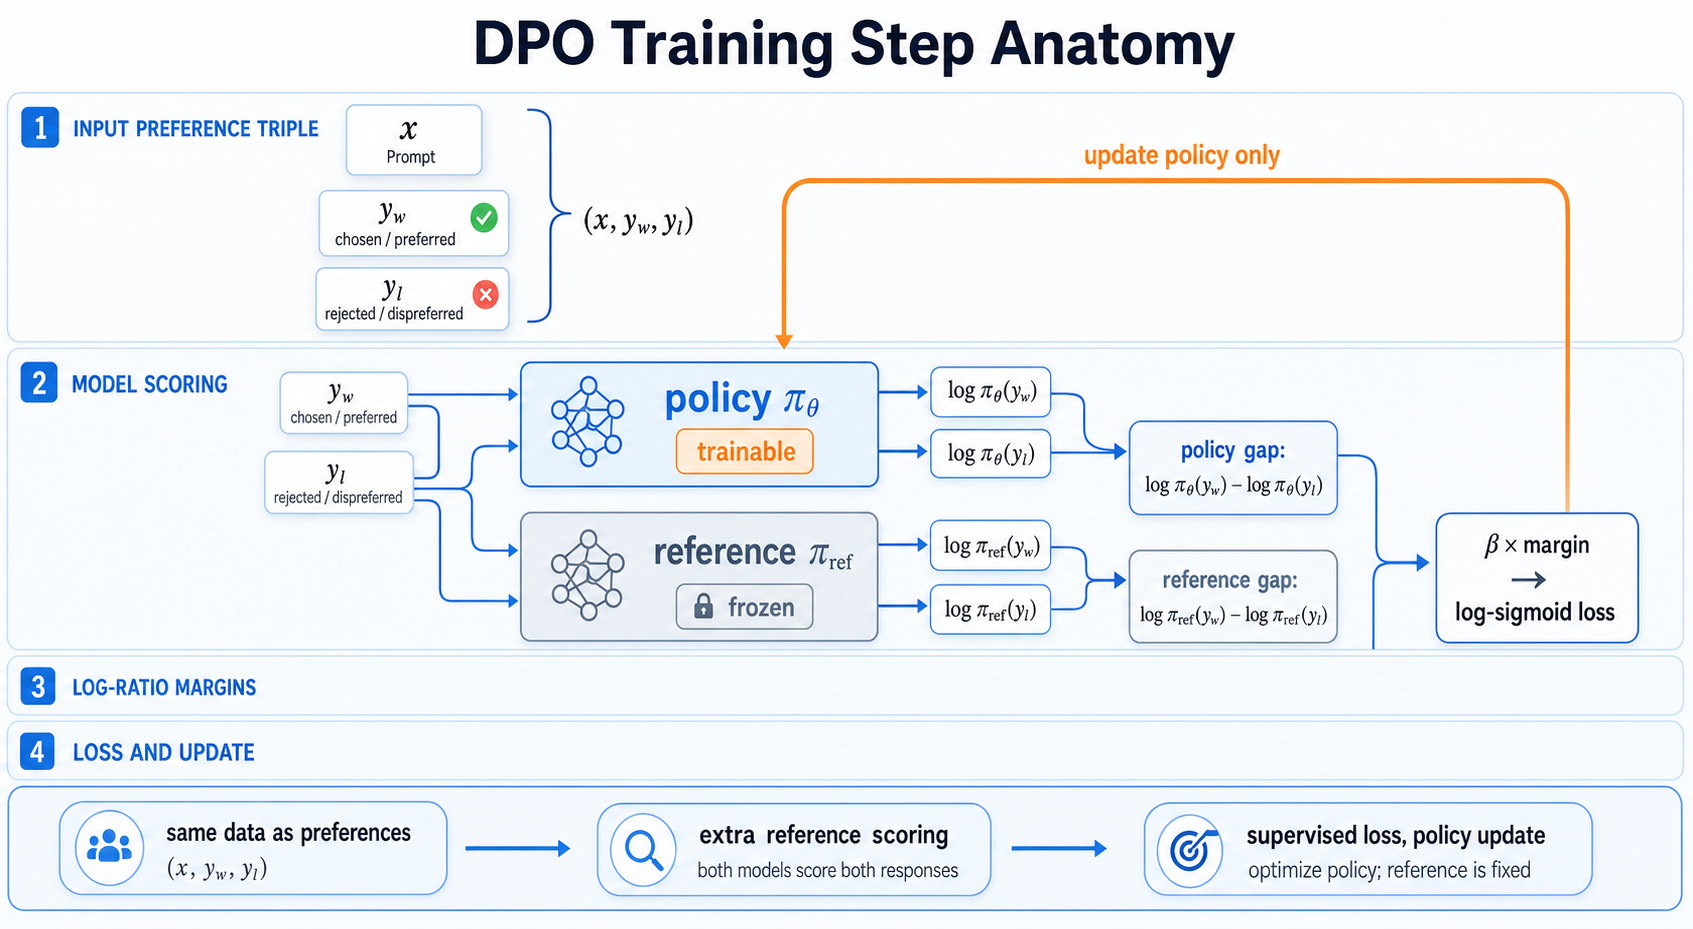
\includegraphics[width=0.95\textwidth]{figures/ch13/fig_dpo_training_step.png}
\caption{\textbf{Anatomy of one DPO training step.} A preference triple $(x,y_w,y_l)$ is scored under both the trainable policy and the frozen reference. DPO compares the policy's winner--loser log-probability gap against the reference gap, scales the margin by $\beta$, and updates only the policy. The figure shows why DPO is supervised in form but still requires careful model bookkeeping.}
\label{fig:dpo-training-step}
\end{figure}

\subsection{The Role of the Reference Model}

The reference model $\pi_{\text{ref}}$ serves two purposes:

\begin{enumerate}[nosep]
  \item \textbf{Anchoring.} The log-ratios measure how much the policy has changed \emph{relative to the starting point}. Without the reference, the loss would depend on the absolute log-probabilities, which are sensitive to response length and tokenization.
  \item \textbf{Regularization.} The reference implicitly enforces the KL constraint from Equation~\ref{eq:kl-objective}. If $\pi_\theta$ diverges too far from $\pi_{\text{ref}}$, the log-ratios grow large, making the gradient signal noisier and the training less stable.
\end{enumerate}

In practice, $\pi_{\text{ref}}$ is the SFT checkpoint from Chapter~\ref{ch:instruction-tuning}---frozen, loaded once, and used only for forward passes. With LoRA (Chapter~\ref{ch:peft}), many implementations can share the same base weights between the reference and the policy adapter. This does not make DPO free: sequence length, batch size, activation memory, and whether reference logits are cached still matter. But it changes the dominant cost from ``two trainable model copies'' to ``one base plus adapter and extra forward passes.''

\subsection{\texorpdfstring{The $\beta$ Hyperparameter}{The beta Hyperparameter}}

$\beta$ controls how aggressively the policy departs from the reference. Practical guidance:

\begin{itemize}[nosep]
  \item \textbf{Typical range}: $\beta \in [0.05, 0.5]$. The original DPO paper used $\beta = 0.1$ as a default.
  \item \textbf{Too small}: the policy optimizes aggressively, risking reward hacking against the implicit reward and mode collapse.
  \item \textbf{Too large}: the policy barely moves from the SFT checkpoint---training is stable but the preference signal has little effect.
  \item \textbf{Practical rule}: start with $\beta = 0.1$, increase if training is unstable, decrease if the model does not improve over the SFT baseline.
\end{itemize}

\begin{tcolorbox}[colback=orange!5, colframe=orange!60, title=\textbf{For Project~3: DPO Training Setup}]
\begin{itemize}[nosep]
  \item Reference model: your SFT checkpoint from Chapter~\ref{ch:instruction-tuning}.
  \item Policy model: same checkpoint, with a new LoRA adapter (Chapter~\ref{ch:peft}).
  \item Preference data: 5K--20K preference pairs. These can be human-annotated, AI-judged, or a mixture.
  \item Hyperparameters: $\beta = 0.1$, learning rate $5 \times 10^{-7}$ to $5 \times 10^{-6}$, 1--3 epochs.
  \item Memory: with QLoRA, policy and reference can share the 4-bit base in common implementations. A 3B model is a realistic single-24\,GB-GPU target if sequence length and batch size are kept modest.
\end{itemize}
\end{tcolorbox}

\begin{quickrecap}
\textbf{Quick Recap.}
\begin{itemize}[nosep,leftmargin=1.5em]
  \item A standard DPO step scores both winner and loser responses under the policy and the reference. Some implementations cache reference log-probabilities; without caching, this is effectively four sequence-scoring passes.
  \item The reference model anchors the log-ratios and implicitly enforces the KL constraint.
  \item $\beta$ is the critical hyperparameter: $\beta = 0.1$ is a robust starting point.
  \item With LoRA/QLoRA, DPO is memory-efficient: policy and reference share the base.
\end{itemize}
\textit{Next: what happens when DPO's assumptions don't hold?}
\end{quickrecap}


%----------------------------------------------------------------------
\section{DPO Failure Modes}
\label{sec:dpo-failures}

DPO's derivation is clean, but its training dynamics have failure modes that are not obvious from the loss function.

\subsection{Likelihood Displacement}

The most counterintuitive empirical finding about DPO: during training, the log-probability of the \emph{preferred} response can \emph{decrease}---not just the dispreferred one~\cite{pal2024smaug, razin2024likelihood}. Both $\log \pi_\theta(y_w \mid x)$ and $\log \pi_\theta(y_l \mid x)$ may drop; the DPO loss only enforces that the \emph{gap} between them grows, not that either one increases in absolute terms.

Why does this happen? The DPO loss (Equation~\ref{eq:dpo-loss}) depends only on the \emph{difference} of log-ratios. As long as the margin $\log [\pi_\theta(y_w)/\pi_{\text{ref}}(y_w)] - \log [\pi_\theta(y_l)/\pi_{\text{ref}}(y_l)]$ increases, the loss decreases---even if both numerators shrink. In effect, DPO can ``prefer'' $y_w$ by pushing $y_l$ down faster than $y_w$, rather than by pushing $y_w$ up.

This matters most when $y_w$ and $y_l$ are similar at the token level (e.g., minor edits to the same response). The model struggles to increase the margin without displacing probability from both. The practical consequence: DPO can reduce the absolute quality of the policy's generations even while ``improving'' according to its own loss. DPO-Positive (DPOP) is one targeted response: it adds pressure to preserve or increase the likelihood of preferred examples, rather than only enlarging the winner--loser margin~\cite{pal2024smaug}.

\subsection{Sensitivity to Noisy Preferences}

A reward model aggregates thousands of preference pairs into a single scalar function, which provides implicit averaging over annotation noise. DPO trains the policy directly on individual preference pairs---noise in any single pair propagates directly into the policy gradient. This makes DPO more sensitive to label noise than reward model training.

When preference labels are noisy (low inter-annotator agreement, ambiguous comparisons, systematic biases from \S\ref{sec:preference-quality}), DPO can overfit to the noise rather than the signal. This is a central motivation for IPO (\S\ref{sec:dpo-variants}), which limits how far the model can push the margin on any single pair.

\subsection{Reference Model Sensitivity}

The reference model $\pi_{\text{ref}}$ is typically the SFT checkpoint, but this choice is not neutral. A stronger SFT model provides a tighter anchor, which constrains the policy to stay closer to a higher-quality starting point. A weaker SFT model provides more room to move---but also more room to move in bad directions. The same preference dataset can produce meaningfully different DPO outcomes depending on the reference quality.

\begin{quickrecap}
\textbf{Quick Recap.}
\begin{itemize}[nosep,leftmargin=1.5em]
  \item Likelihood displacement: DPO can decrease the probability of \emph{both} preferred and dispreferred responses, as long as the margin grows.
  \item DPO is more sensitive to noisy preferences than reward model training, because noise enters the policy gradient directly.
  \item Reference model quality meaningfully affects DPO outcomes; a stronger SFT checkpoint anchors better.
\end{itemize}
\textit{Next: variants of DPO that address these failure modes.}
\end{quickrecap}


%----------------------------------------------------------------------
\section{DPO Variants}
\label{sec:dpo-variants}

The failure modes in the previous section motivate several DPO variants. Each modifies a specific assumption or addresses a specific weakness.

\subsection{IPO (Identity Preference Optimization)}

IPO~\cite{azar2024ipo} directly addresses the likelihood displacement problem from \S\ref{sec:dpo-failures}. The core insight: DPO's sigmoid loss has no finite target margin. When the preference is effectively deterministic, the unregularized optimum pushes the winner--loser margin toward infinity; the gradient becomes small as the margin grows, but the objective still favors ever-larger separation. This can amplify likelihood displacement on easy or noisy pairs.

IPO replaces the log-sigmoid with a squared loss that targets a \emph{finite} margin:
%
\[
\mathcal{L}_{\text{IPO}}(\theta) = \mathbb{E}\!\left[\left(\log \frac{\pi_\theta(y_w \mid x)}{\pi_{\text{ref}}(y_w \mid x)} - \log \frac{\pi_\theta(y_l \mid x)}{\pi_{\text{ref}}(y_l \mid x)} - \frac{1}{2\beta}\right)^{\!2}\right]
\]
%
The squared penalty prevents the margin from growing without bound. On noisy preference data, this makes IPO more robust than DPO: the model converges to a moderate margin rather than overfitting the noise.

\subsection{SimPO (Simple Preference Optimization)}

SimPO~\cite{meng2024simpo} removes the reference model entirely. Instead of comparing log-ratios against a frozen reference, SimPO uses the \emph{length-normalized} log-probability of each response as the implicit reward:
%
\[
\mathcal{L}_{\text{SimPO}}(\theta) = -\mathbb{E}\!\left[\log \sigma\!\left(\frac{\beta}{|y_w|} \log \pi_\theta(y_w \mid x) - \frac{\beta}{|y_l|} \log \pi_\theta(y_l \mid x) - \gamma\right)\right]
\]
%
where $|y|$ is response length and $\gamma$ is a target margin. Length normalization directly addresses the length bias from \S\ref{sec:preference-quality}: without it, longer responses accumulate more log-probability simply by having more tokens.

SimPO's appeal is operational: no reference model in memory, no reference forward passes, and built-in length-bias mitigation. By 2024--2025, SimPO became a practical alternative for open-model preference tuning.

\subsection{KTO (Kahneman-Tversky Optimization)}

KTO~\cite{ethayarajh2024kto} drops the pairwise requirement entirely. Instead of preference pairs $(y_w, y_l)$, KTO uses only \emph{individual} responses labeled as ``good'' or ``bad.'' This is useful when pairwise data is expensive or unavailable---you only need thumbs-up / thumbs-down labels. The loss is derived from Kahneman and Tversky's prospect theory, treating gains (good responses) and losses (bad responses) asymmetrically. The trade-off: KTO uses less informative data (one bit per response rather than one bit per pair), so it typically requires more examples to match DPO's quality.

\subsection{ORPO (Odds Ratio Preference Optimization)}

ORPO~\cite{hong2024orpo} combines the SFT and preference losses into a single objective: the SFT loss on preferred responses plus a preference term based on the odds ratio. The benefit is simplicity---no separate SFT and DPO stages, no reference model. The risk is that combining two objectives with different learning dynamics can require careful balancing.

\paragraph{Which variant to use?}

\begin{itemize}[nosep]
  \item \textbf{DPO}: the default. Best understood, most widely validated, broadest ecosystem support.
  \item \textbf{IPO}: when preference data is noisy or when DPO overfits by driving margins to infinity (\S\ref{sec:dpo-failures}).
  \item \textbf{SimPO}: when you want to drop the reference model and mitigate length bias simultaneously.
  \item \textbf{KTO}: when you only have per-response quality labels, not paired comparisons.
  \item \textbf{ORPO}: when you want to eliminate the separate SFT stage (experimental; less mature than DPO).
\end{itemize}

\begin{figure}[t]
\centering
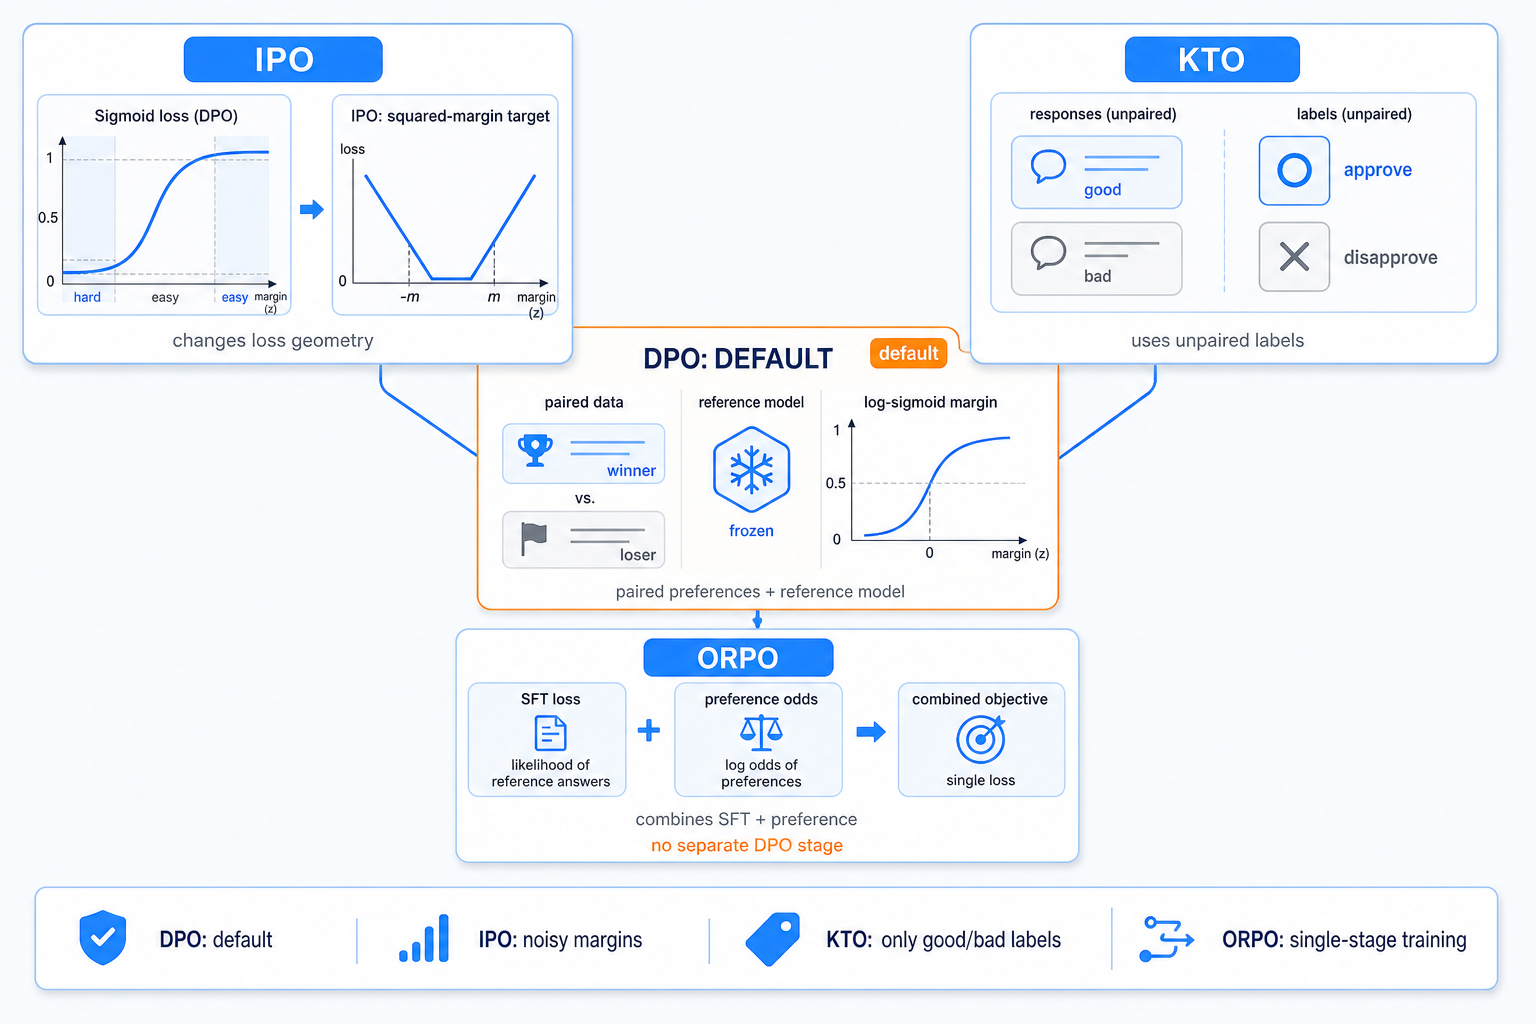
\includegraphics[width=0.95\textwidth]{figures/ch13/fig_dpo_variants.png}
\caption{\textbf{Representative DPO variants modify different assumptions.} DPO sits at the center: paired preferences, a frozen reference, and a log-sigmoid margin loss. IPO changes the loss geometry, KTO changes the data format to unpaired good/bad labels, and ORPO merges SFT and preference learning into one objective. SimPO, discussed in the text, removes the reference model and length-normalizes the implicit reward. The right variant depends on what kind of data and stability problem you actually have.}
\label{fig:dpo-variants}
\end{figure}

\begin{quickrecap}
\textbf{Quick Recap.}
\begin{itemize}[nosep,leftmargin=1.5em]
  \item IPO avoids sigmoid saturation; more robust to noisy data.
  \item SimPO removes the reference model and length-normalizes response log-probability.
  \item KTO works with unpaired good/bad labels instead of preference pairs.
  \item ORPO combines SFT and preference learning in one loss; no reference model needed.
  \item DPO remains the default for most practical applications.
\end{itemize}
\textit{Next: what can DPO handle, and where does it fall short?}
\end{quickrecap}


%----------------------------------------------------------------------
\section{When DPO Suffices, When It Doesn't}
\label{sec:dpo-limits}

DPO is not a universal solution. Understanding its capability boundary is essential for choosing the right tool.

\subsection{Where DPO Excels}

DPO works well when the quality signal is \emph{holistic and comparative}: the annotator (human or AI) can judge the overall quality of a response, and the signal can be expressed as ``A is better than B.''

\begin{itemize}[nosep]
  \item \textbf{Helpfulness}: more complete, more relevant, better structured responses.
  \item \textbf{Format compliance}: following instructions about length, style, structure.
  \item \textbf{Tone and safety}: avoiding harmful, offensive, or evasive responses.
  \item \textbf{Reducing verbosity}: preferring concise responses over unnecessarily long ones (when data collection controls for length bias).
\end{itemize}

\subsection{Where DPO Struggles}

DPO struggles when:

\begin{itemize}[nosep]
  \item \textbf{The reward signal is dense, not holistic.} In math or code, each step matters---but a pairwise preference only says ``this whole response is better.'' It provides no information about \emph{which steps} were good or bad. Process reward models (Chapter~\ref{ch:reasoning-rl}) address this.
  \item \textbf{The model needs to learn new capabilities, not refine existing ones.} DPO fine-tunes the policy relative to the SFT reference. If the SFT model cannot produce a reasonable response to a class of prompts, DPO has no ``better'' response to learn from. DPO sharpens; it does not create.
  \item \textbf{The preference data is far from the policy's distribution.} If the preferred and dispreferred responses in the training data come from a different model or an earlier checkpoint, the log-ratios may be poorly calibrated. Online or iterative DPO (\S\ref{sec:iterative-dpo}) addresses this.
  \item \textbf{Extended reasoning is required.} Tasks like multi-step math, complex code generation, and planning benefit from training signals that reward correct outcomes (verifiable rewards), not just human style preferences. This is the domain of reasoning RL (Chapter~\ref{ch:reasoning-rl}).
\end{itemize}

\begin{figure}[t]
\centering
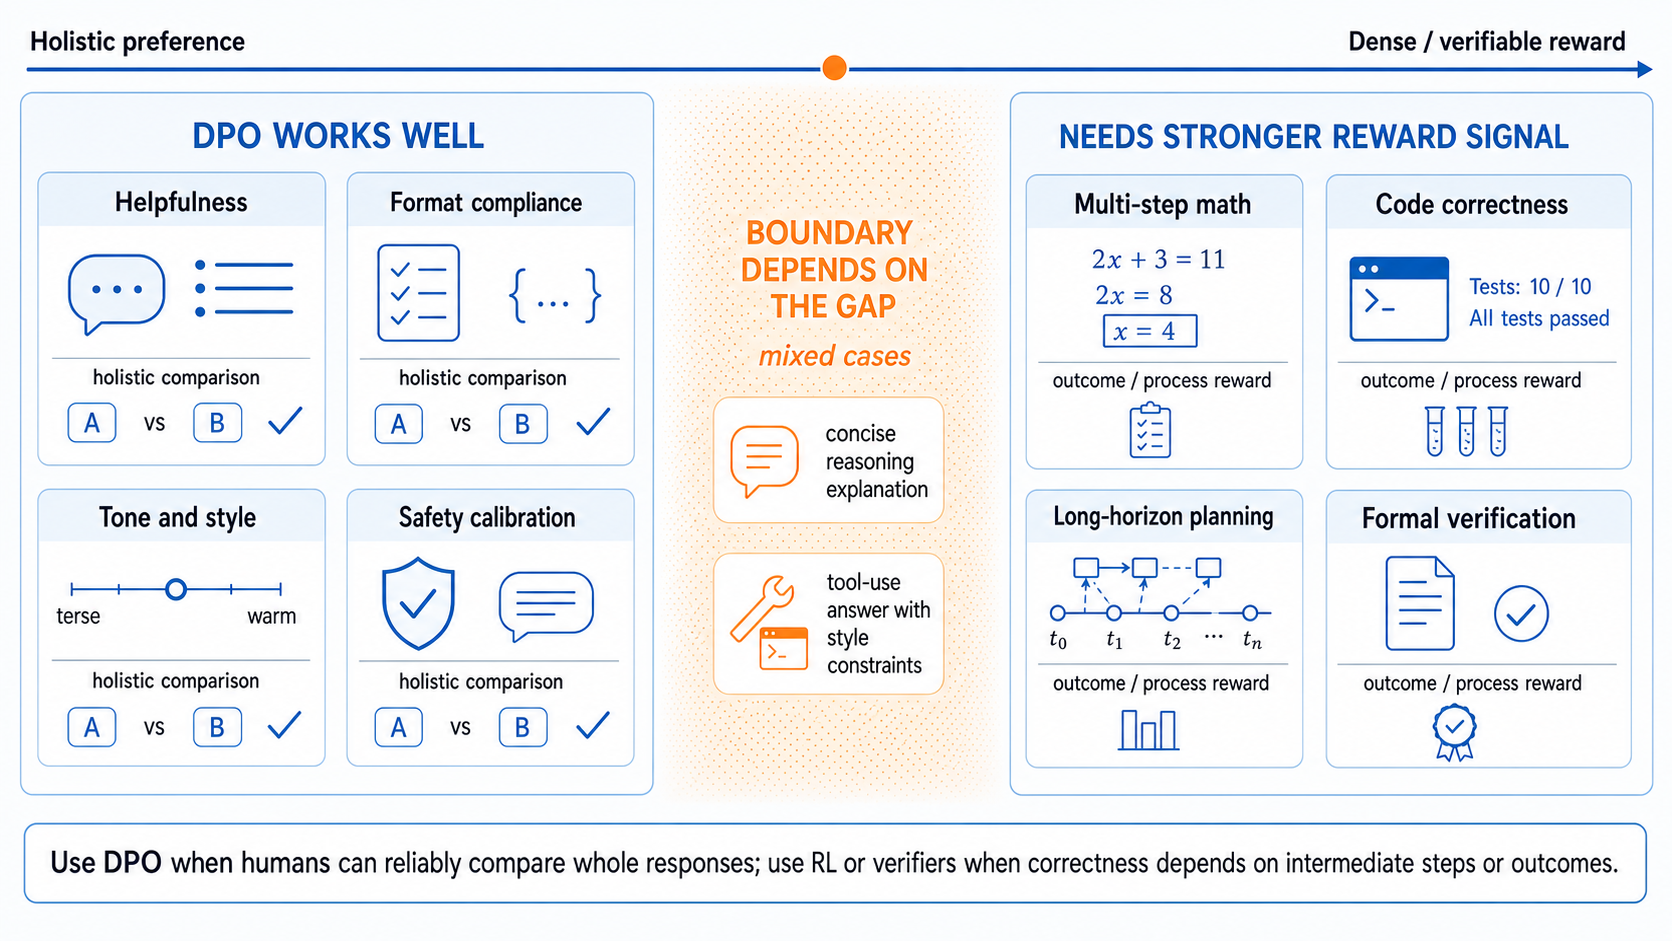
\includegraphics[width=0.95\textwidth]{figures/ch13/fig_dpo_boundary.png}
\caption{\textbf{The DPO capability boundary.} Left: tasks where DPO excels---helpfulness, format, tone, safety---all involve holistic comparative judgments. Right: tasks where DPO struggles---math reasoning, code correctness, sustained planning---all require dense or outcome-based reward signals. The boundary is not sharp: many tasks fall in between, and the right method depends on the specific quality gap.}
\label{fig:dpo-boundary}
\end{figure}

\begin{quickrecap}
\textbf{Quick Recap.}
\begin{itemize}[nosep,leftmargin=1.5em]
  \item DPO excels at holistic quality improvements: helpfulness, format, tone, safety.
  \item DPO struggles with dense reward signals (step-by-step correctness) and capability creation (tasks the SFT model cannot do at all).
  \item For reasoning and code, verifiable reward RL (Chapter~\ref{ch:reasoning-rl}) is the better tool.
\end{itemize}
\textit{Next: can you improve DPO by collecting preferences iteratively?}
\end{quickrecap}


%----------------------------------------------------------------------
\section{Iterative DPO and Multi-Round Preference Training}
\label{sec:iterative-dpo}

Standard (``offline'') DPO trains on a fixed preference dataset collected before training begins. The preferred and dispreferred responses typically come from the SFT model or an earlier checkpoint. As the policy improves during training, it may move far from the distribution that generated the training data, making the log-ratios less informative. This is the \textbf{distribution shift problem}: the policy learns to distinguish responses it would never generate.

\subsection{Online DPO}

The fix: generate new preference pairs from the \emph{current} policy during training. After every $k$ optimization steps, sample new responses from $\pi_\theta$, collect preferences (from an RM or AI judge), and add these to the training batch. The preference data stays on-distribution because the policy generates it.

Online DPO is more expensive---it requires repeated inference and annotation during training---but it avoids the stale-data problem. Empirically, online DPO tends to produce stronger models than offline DPO for the same data budget.

\subsection{Iterative DPO}

A simpler approximation: train DPO to convergence on the initial preference dataset, then generate new preference data from the trained model, and train a second round of DPO starting from the first round's output. This can be repeated for multiple rounds. Each round uses on-policy data for that round's starting point, reducing (but not eliminating) distribution shift.

The risk of iterative DPO is \textbf{preference collapse}: if the preference data is generated by an AI judge, and the AI judge favors the policy's current style, iterative training amplifies that style rather than genuinely improving. Diversity in the prompt set and the judge are important safeguards.

\paragraph{The RL boundary.} Notice what online DPO has reintroduced: an inference loop (sample from the current policy), a reward signal (judge the samples), and iterative on-policy training (update the policy, re-sample, repeat). These are the operational components of RL---the only thing that differs is the gradient step, which uses the DPO loss rather than a policy gradient estimator. Offline DPO genuinely ``skips RL''---it trains on a fixed dataset with a supervised loss. Online DPO sits on the boundary: supervised in its loss function, but RL-like in its data pipeline. This observation will sharpen in Chapter~\ref{ch:rl-foundations}, where the RL view of preference optimization makes the connection explicit.

\begin{quickrecap}
\textbf{Quick Recap.}
\begin{itemize}[nosep,leftmargin=1.5em]
  \item Offline DPO suffers from distribution shift: the policy outgrows its training data.
  \item Online DPO generates fresh preference pairs from the current policy during training.
  \item Iterative DPO trains multiple rounds, each starting from the previous round's model.
  \item Both mitigate distribution shift but add cost and risk preference collapse with AI judges.
  \item Online DPO reintroduces most operational components of RL. The ``no RL'' framing applies cleanly only to offline DPO.
\end{itemize}
\textit{Next: where does all of this stand in industry practice?}
\end{quickrecap}


%----------------------------------------------------------------------
\section{Industry Reality}
\label{sec:preference-industry}

The 2024--2025 open-source landscape converged on a practical default: \textbf{SFT + DPO-style preference tuning}. Models and recipes such as Zephyr, Tulu-style training, OpenChat-like fine-tunes, and numerous Llama/Mistral derivatives use this family of methods because it is simple, stable, and compatible with PEFT. Full RLHF (RM + PPO) remains important, but it is no longer the default path for most open-model fine-tuning work.

\paragraph{Why DPO won the open-source default.}

\begin{itemize}[nosep]
  \item \textbf{Simplicity}: one loss function, two models (one frozen), no RL loop.
  \item \textbf{Memory efficiency}: with LoRA, policy and reference share a base (Chapter~\ref{ch:peft}).
  \item \textbf{Stability}: DPO training is more predictable than PPO. Fewer catastrophic runs.
  \item \textbf{Quality}: on common alignment benchmarks such as AlpacaEval and MT-Bench, DPO-style methods often provide most of the helpfulness and format gains practitioners want from preference tuning.
\end{itemize}

\paragraph{Where RLHF is still used.}

\begin{itemize}[nosep]
  \item \textbf{Frontier alignment}: large labs still invest in reward modeling and RL-style training for safety-critical alignment properties where the additional control of RM + PPO can matter.
  \item \textbf{Reasoning capabilities}: reasoning RL (Chapter~\ref{ch:reasoning-rl}) uses verifiable rewards, not human preferences. This is a different application of RL, not classical RLHF.
  \item \textbf{Nuanced trade-offs}: when the alignment signal involves complex trade-offs between helpfulness and safety, the reward model provides a more granular signal than DPO's pairwise loss.
\end{itemize}

\paragraph{The honest framing.} The choice between DPO and RLHF is not ``DPO is better.'' It is: DPO is \emph{sufficient} for most open-source use cases, and its operational simplicity makes it the rational default. RLHF is a more powerful tool that requires more infrastructure. For Project~3 and most academic work, DPO is the right choice.

\begin{quickrecap}
\textbf{Quick Recap.}
\begin{itemize}[nosep,leftmargin=1.5em]
  \item SFT + DPO is the 2024--2025 open-source default.
  \item Full RLHF remains important for frontier-scale alignment and safety-critical applications.
  \item DPO's advantage is operational simplicity and stability, not theoretical superiority.
  \item For Project~3: use DPO.
\end{itemize}
\end{quickrecap}


%----------------------------------------------------------------------
% KEY TAKEAWAYS
%----------------------------------------------------------------------
\begin{takeaways}
\textbf{Key Takeaways}
\begin{itemize}[nosep]
  \item Pairwise preferences are more reliable and cognitively simpler than absolute scores, making them the dominant annotation format for alignment.
  \item The Bradley-Terry model converts pairwise comparisons into a scalar reward signal via logistic regression on reward differences.
  \item A reward model is a language model with a scalar head, trained on the Bradley-Terry loss. It achieves 65--75\% agreement with human preferences---close to the human-human agreement ceiling.
  \item The KL-constrained preference objective balances reward maximization against policy drift. Its closed-form solution is the reference policy reweighted by exponentiated reward.
  \item DPO eliminates the reward model and RL loop entirely: a supervised loss on preference pairs, derived from the KL-constrained objective by canceling the intractable partition function. A trained DPO policy implicitly encodes a reward function---your language model is secretly a reward model.
  \item DPO has its own failure modes: likelihood displacement (both preferred and dispreferred probabilities can decrease), sensitivity to noisy preferences, and dependence on reference model quality.
  \item DPO excels at holistic quality improvements (helpfulness, format, tone, safety) but struggles with dense reward signals (step-by-step reasoning) and capability creation.
  \item SFT + DPO is the 2024--2025 open-source default. Full RLHF is justified for frontier alignment and reasoning RL.
\end{itemize}
\end{takeaways}


%----------------------------------------------------------------------
\section*{Summary}

\paragraph{What this chapter established.} Preference learning transforms alignment from an imitation problem to a comparison problem. Instead of showing the model what to say, you show it which of two responses is better. The Bradley-Terry model gives this comparison a mathematical foundation; the reward model makes it scalable; DPO makes it simple. By the end of the chapter, you have a complete pipeline from preference annotation to model update---and it runs as a supervised loss.

\paragraph{The comparison-to-gradient lesson.} The most important idea in this chapter is not the DPO loss function---that is a formula. It is the realization that \emph{comparison is a different signal than demonstration}. A demonstration says ``imitate this.'' A comparison says ``prefer this response over that one.'' DPO's derivation shows that this comparative signal can be extracted without the machinery of RL: the KL-constrained objective has a closed-form solution, and the partition function cancels in pairwise comparisons. The entire reward model plus RL pipeline collapses to supervised learning---\emph{if} you have the right data format. And a deeper insight: the trained policy is not merely aligned---it secretly encodes the reward function itself, enabling best-of-N sampling and rejection sampling without a separate reward model.

\paragraph{One sentence.} You do not need RL to learn from preferences---the KL-constrained objective has a closed-form policy, and DPO extracts its gradient from preference pairs alone.

\paragraph{What comes next.} Chapter~\ref{ch:rl-foundations} builds the RL vocabulary you need for Chapters~\ref{ch:rlhf}--\ref{ch:reasoning-rl}: MDPs, policy gradients, PPO. When you reach the KL-constrained objective there, you will recognize it from this chapter---but now derived from RL principles rather than optimization.


%----------------------------------------------------------------------
\section*{Key Equations at a Glance}

\begin{center}
\begin{tabularx}{\textwidth}{@{}p{5cm}X@{}}
\toprule
\textbf{Quantity} & \textbf{Expression} \\
\midrule
Bradley-Terry preference & $P(y_w \succ y_l \mid x) = \sigma\!\bigl(r(x, y_w) - r(x, y_l)\bigr)$ \\[4pt]
RM training loss & $\mathcal{L}_{\text{BT}} = -\mathbb{E}\bigl[\log \sigma\!\bigl(r_\phi(y_w) - r_\phi(y_l)\bigr)\bigr]$ \\[4pt]
KL-constrained objective & $\max_{\pi} \;\mathbb{E}[r(x,y)] - \beta\, D_{\text{KL}}[\pi \| \pi_{\text{ref}}]$ \\[4pt]
Optimal policy & $\pi^*(y \mid x) = \frac{1}{Z(x)}\,\pi_{\text{ref}}(y \mid x)\,\exp\!\bigl(r(x,y)/\beta\bigr)$ \\[4pt]
DPO loss & $\mathcal{L}_{\text{DPO}} = -\mathbb{E}\!\left[\log \sigma\!\left(\beta \log \frac{\pi_\theta(y_w)}{\pi_{\text{ref}}(y_w)} - \beta \log \frac{\pi_\theta(y_l)}{\pi_{\text{ref}}(y_l)}\right)\right]$ \\
\bottomrule
\end{tabularx}
\end{center}


%----------------------------------------------------------------------
\section*{Key Readings}

\begin{enumerate}[nosep]
  \item \textbf{Ouyang et al., 2022.} ``Training Language Models to Follow Instructions with Human Feedback'' (InstructGPT). The production-scale three-stage pipeline. Read for the RLHF baseline that DPO simplifies.
  \item \textbf{Rafailov et al., 2023.} ``Direct Preference Optimization: Your Language Model Is Secretly a Reward Model'' (DPO). The core paper for this chapter. The derivation is accessible; the experiments on TL;DR summarization are clean.
  \item \textbf{Bai et al., 2022.} ``Training a Helpful and Harmless Assistant with Reinforcement Learning from Human Feedback.'' Anthropic's preference data methodology and Constitutional AI. Read for the data pipeline, not just the algorithm.
  \item \textbf{Christiano et al., 2017.} ``Deep Reinforcement Learning from Human Preferences.'' The foundational work connecting human preferences to RL. Short and readable; establishes the conceptual framework.
  \item \textbf{Azar et al., 2024.} ``A General Theoretical Paradigm to Understand Learning from Human Feedback'' (IPO). The most important DPO variant paper. Read for the analysis of DPO's failure modes and the IPO fix.
  \item \textbf{Ethayarajh et al., 2024.} ``KTO: Model Alignment as Prospect Theoretic Optimization.'' Drops the pairwise requirement entirely. Read if you have per-response quality labels instead of preference pairs.
  \item \textbf{Gao et al., 2023.} ``Scaling Laws for Reward Model Overoptimization.'' Documents the Goodhart's law dynamic in reward model optimization. Essential for understanding why KL constraints matter.
\end{enumerate}

\flushbottom
